\documentclass{article}


\usepackage{lmodern}
\usepackage[T1]{fontenc}
\usepackage[spanish,activeacute]{babel}
\usepackage{mathtools}
\usepackage{subfig}
\usepackage{graphicx}
\usepackage{listings}
\usepackage{float}

\begin{document}

\begin{figure}[htbp]

\includegraphics{logo_latex} 
\end{figure}

\textbf{\Huge{Informe de Tarea \#3}}\\[0.2cm]
\textbf{\Huge{Redes de Computadores}}
\\ \ \\ \

\begin{flushleft}
\large{\textbf{Profesor:}} 
\large{Oscar Encina Calqu'in} 
\\ \


\large{\textbf{Integrantes:}} \par
\large{Felipe Araya Barrera  201173501-3  felipe.araya@alumnos.usm.cl}\\ \

\large{Felipe Berrios Toloza  201173501-3 felipe.berrios@alumnos.usm.cl}\\

\end{flushleft}

\newpage

\section{Introducci'on}
En el siguiente informe se trabajar'a sobre la capa de red, para ello se utilizar'a el programa Open Visual Traceroute el cual nos permitir'a rastrear la ruta de un paquete de datos desde la ubicaci'on del env'io hasta el servidor de destino.

\section{Recorrido de los paquetes}
En primer punto se usar'a OVT para observar que sucede con las direcciones escogidas. El servidor de inicio ser'a el de mi hogar:

\subsection{http://moodle.inf.usm.cl/}
Primero se revisar'a el recorrido del link del moodle de nuestra universidad:
\\
\begin{figure}[H]
  \centering
    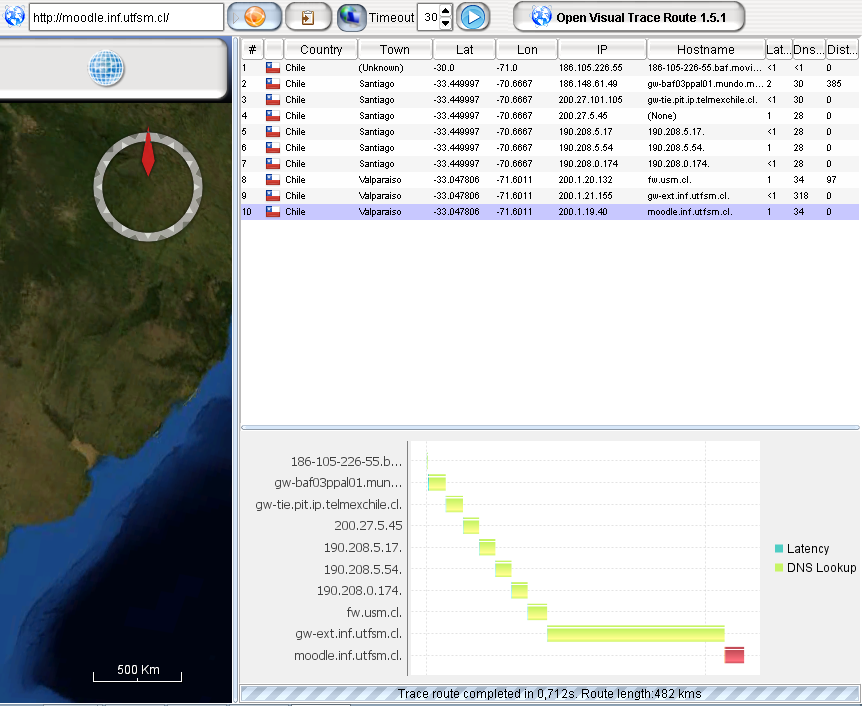
\includegraphics[width=1.0\textwidth]{ruta1_moodle}
  \caption{Recorrido link Moodle}
  \label{moodle}
\end{figure}\\

El tiempo del recorrido de la ruta dura 0,712 segundos con un recorrido total en orden desde Santiago a Valparaíso de 482 kil'ometros.

\subsection{http://google.cl/}
Luego se proceder'a a revisar el recorrido hecho por el buscador Google:
\\
\begin{figure}[H]
  \centering
    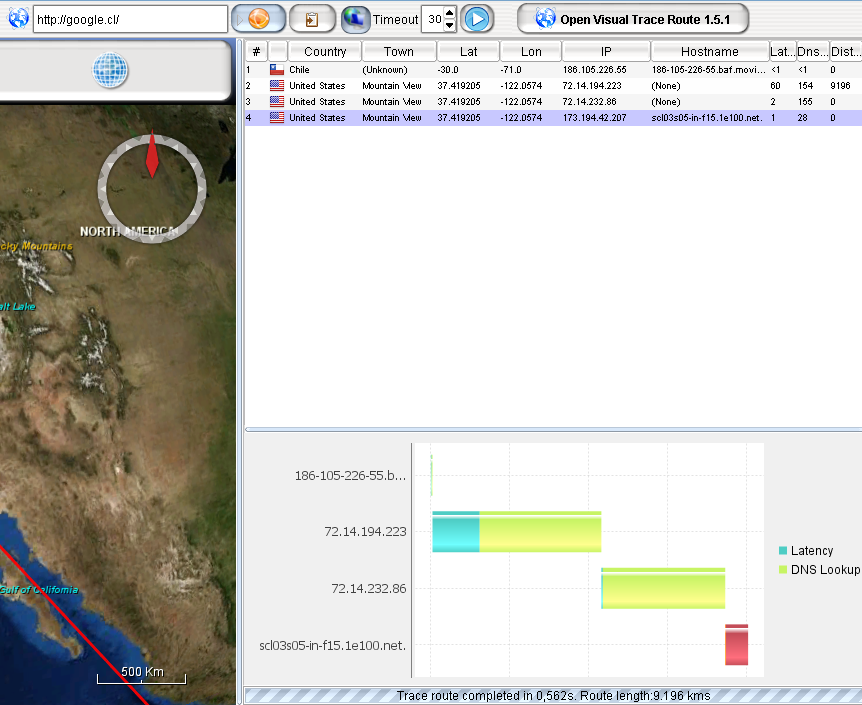
\includegraphics[width=1.0\textwidth]{ruta1_google}
  \caption{Recorrido link Google}
  \label{google}
\end{figure}\\

El tiempo del recorrido de la ruta dura 0,562 segundos con un recorrido total en orden desde Santiago a Mountain View de 9.196 kilómetros.

\subsection{http://cime.cl/}
La tercera página a revisar ser'a la del Cime:
\\
\begin{figure}[H]
  \centering
    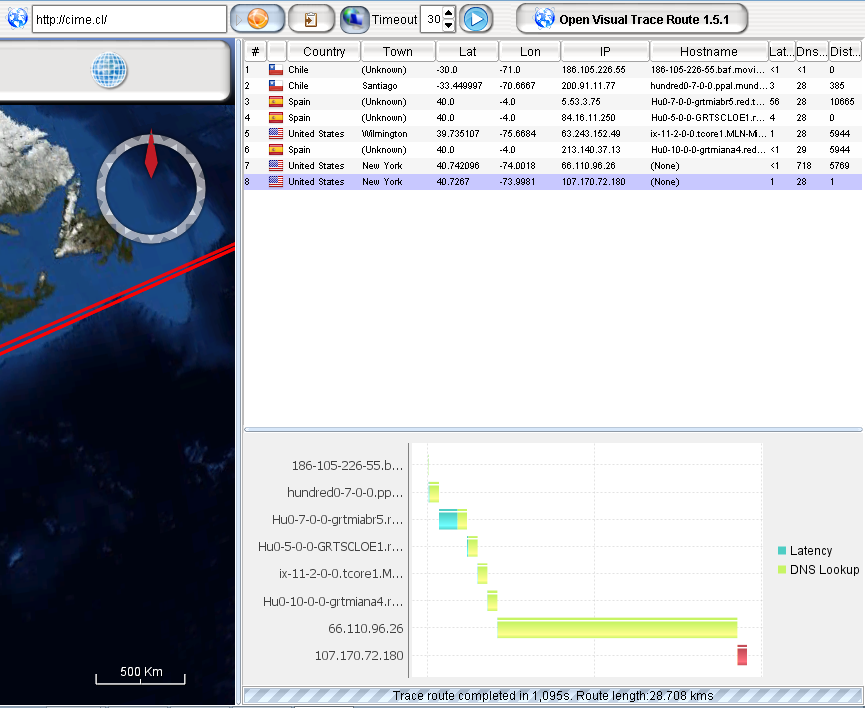
\includegraphics[width=1.0\textwidth]{ruta1_cime}
  \caption{Recorrido link Cime}
  \label{cime}
\end{figure}\\

El tiempo del recorrido de la ruta dura 1,095 segundos con un recorrido total en orden desde Santiago a España, Estados Unidos, nuevamente a España, regresando finalmente a Estados Unidos de 28.708 kil'ometros.

\subsection{http://wikipedia.com/}
El recorrido de Wikipedia es el siguiente:
\\
\begin{figure}[H]
  \centering
    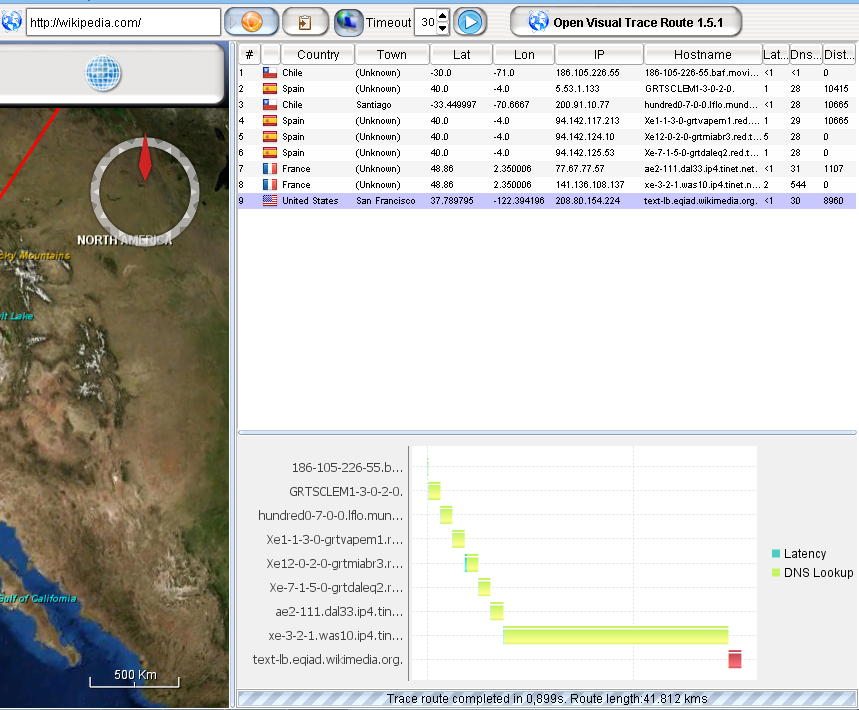
\includegraphics[width=1.0\textwidth]{ruta1_wikipedia}
  \caption{Recorrido link Wikipedia}
  \label{wikipedia}
\end{figure}\\

El tiempo del recorrido de la ruta dura 0,899 segundos con un recorrido total en orden desde Santiago a España, regreso a Chile, nuevamente a España, luego pasando por Francia y finalmente a San Francisco, Estados Unidos de 41.812 kil'ometros.

\subsection{http://www.chile.embassy.gov.au/}
El recorrido de la p'agina de la embajada de Chile en Australia es el siguiente:
\\
\begin{figure}[H]
  \centering
    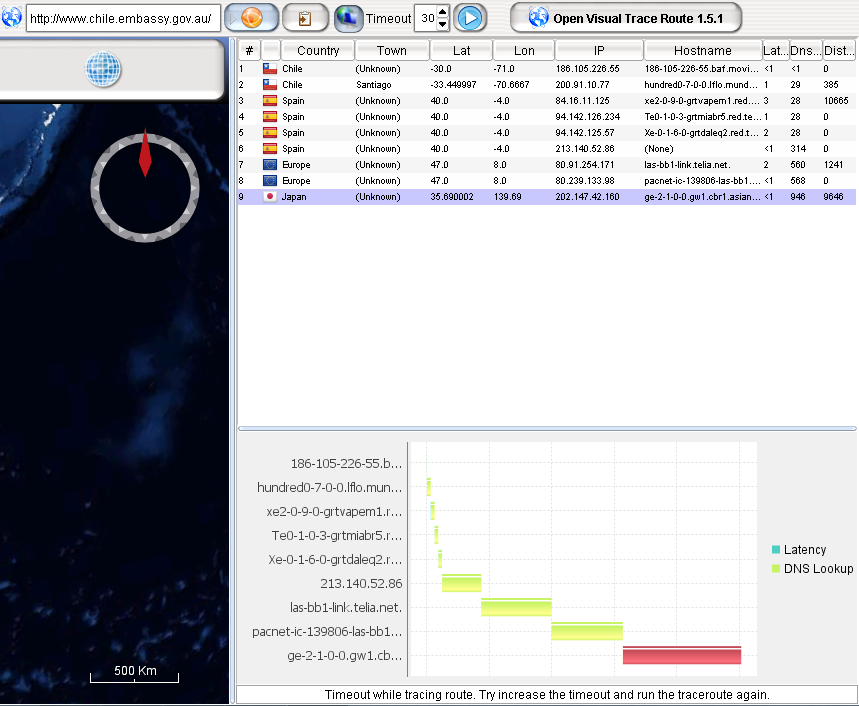
\includegraphics[width=1.0\textwidth]{ruta1_embchile}
  \caption{Recorrido link Embajada chilena en Australia}
  \label{embchile}
\end{figure}\\

Este recorrido tiene la peculiaridad de que despu'es de 30 segundos el recorrido llega a timeout, donde no llega al servidor destino, pese a que el paquete de datos viaja por Santiago, España, una localidad de Europa y luego Jap'on.\\ \

En primera instancia, se aprecia que las rutas se realizan generalmente en tiempos muy cortos, adem'as llama la atenci'on que el tiempo del recorrido de la p'agina de Google es menor a la del moodle de nuestra universidad, considerando la gran distancia que hay entre pa'ises. Todo eso se ver'a con m'as profundidad en el siguiente punto.

\section{Los paquetes y las rutas}









\end{document}